\documentclass{article} % For LaTeX2e
\usepackage{nips15submit_e,times}
\usepackage{hyperref}
\usepackage{url}
%\documentstyle[nips14submit_09,times,art10]{article} % For LaTeX 2.09

\usepackage{hyperref}
\usepackage{url}
\usepackage[utf8x]{inputenc}
\usepackage[english]{babel}
\usepackage{algorithm}
\usepackage{algorithmic}
\usepackage{amsfonts}
\usepackage{graphics}
\usepackage{graphicx}
\usepackage{tikz}
\usetikzlibrary{bayesnet}
\tikzstyle{connect}=[-latex, thick]
\tikzstyle{allconnected}=[line width=0.15cm]

%\usepackage{verbatim}
%\usepackage[active,tightpage]{preview}
%\PreviewEnvironment{tikzpicture}
%\usepackage{savetrees}

\def\bbbr{{\rm I\!R}}
\newcommand{\vp}{\vec{\phi}}
\newcommand{\vmu}{\vec{\mu}}
\newcommand{\vf}{\vec{f}}
\newcommand{\vw}{\vec{w}}
\newcommand{\vm}{\vec{m}}
\newcommand{\vx}{\vec{x}}
\newcommand{\vr}{\vec{r}}
\newcommand{\vy}{\vec{y}}
\newcommand{\vz}{\vec{z}}
\newcommand{\vY}{\vec{Y}}
\newcommand{\vX}{\vec{X}}
\newcommand{\bx}{\textbf{x}}
\newcommand{\bw}{\textbf{w}}
\newcommand{\by}{\textbf{y}}
\newcommand{\bL}{\textbf{L}}
\newcommand{\bI}{\textbf{I}}
\newcommand{\vk}{\vec{k}}
\newcommand{\vL}{\vec{\Lambda}}
\newcommand{\xmin}{x_{\min}}
\newcommand{\pmin}{p_{\min}}
\newcommand{\fmin}{f_{\min}}
\newcommand{\hpmin}{\hat{p}_{\min}}
\newcommand{\hqmin}{\hat{q}_{\min}}
\newcommand{\pfmin}{p_{f_{\min}}}
\renewcommand{\vec}{\boldsymbol}
\newcommand{\fun}[1]{\mathsf{#1}}
\renewcommand{\O}{\mathcal{O}}
\newcommand{\GP}{\mathcal{GP}}
\newcommand{\N}{\mathcal{N}}
\newcommand{\Id}{\vec{I}}
\newcommand{\II}{\mathbb{I}}
\newcommand{\IR}{\mathbb{R}}

\newcommand{\tr}{\operatorname{tr}}
\newcommand{\argmin}{\operatorname*{arg\: min}}
\newcommand{\argmax}{\operatorname*{arg\: max}}
\newcommand{\chol}{\operatorname{\mathsf{C}}}

\newcommand{\data}{\mathcal{D}}
\newcommand{\xst}{x_{\ast}}
\newcommand{\yst}{y_{\ast}}

\newtheorem{theorem}{Theorem}
\newtheorem{lemma}{Lemma}
\newtheorem{corollary}{Corollary}
\newtheorem{proposition}{Proposition}
\newtheorem{definition}{Definition}
\newtheorem{proof}{Proof}
\newtheorem{conjecture}{Conjecture}





\title{
    GLASSES: Relieving The Myopia Of Bayesian Optimisation
    }
    
 
\author{
David S.~Hippocampus\thanks{ Use footnote for providing further information about author (webpage, alternative address)---\emph{not} for acknowledging funding agencies.} \\
Department of Computer Science\\
Cranberry-Lemon University\\
Pittsburgh, PA 15213 \\
\texttt{hippo@cs.cranberry-lemon.edu} \\
\And
Coauthor \\
Affiliation \\
Address \\
\texttt{email} \\
}

\newcommand{\fix}{\marginpar{FIX}}
\newcommand{\new}{\marginpar{NEW}}

%\nipsfinalcopy % Uncomment for camera-ready version

    
\begin{document}

\maketitle


\abstract{
    We present GLASSES: Global optimisation with Look-Ahead through Stochastic Simulation and Expected-loss Search. Our algorithm tackles the long-standing myopia of Bayesian optimisation approaches.
}

\begin{figure}
\centering
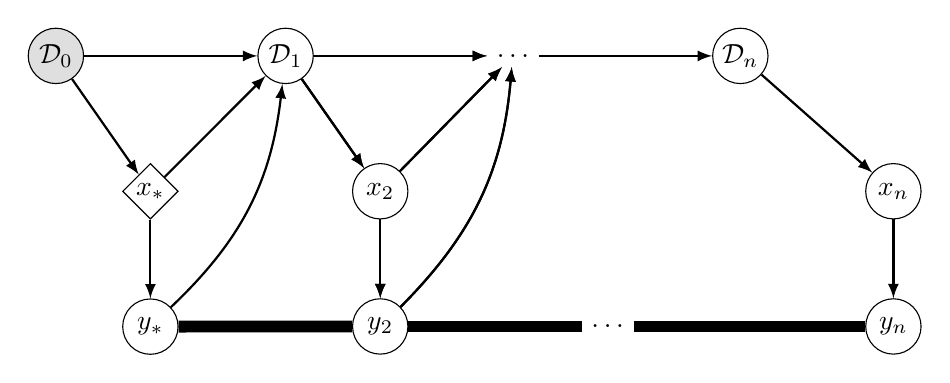
\begin{tikzpicture}

    % first row
    \node[obs] (D0) {$\data_0$};
    \node[latent, right=of D0, xshift=1.2cm] (D1) {$\data_1$};
    \node[draw=none, right=of D1, xshift=1.2cm] (Ddots) {$\ldots$};
    \node[latent, right=of Ddots, xshift=1.2cm] (Dn) {$\data_n$};

    % second row
    \node[det, below=of D0, xshift=1.2cm] (xst) {$\xst$};
    \node[latent, right=of xst, xshift=1.2cm] (x2) {$x_2$};
    \node[latent, right=of x2, xshift=4.8cm] (xn) {$x_n$};

    % third row
    \node[latent, below=of xst] (yst) {$\yst$};
    \node[latent, below=of x2] (y2) {$y_2$};
    \node[draw=none, right=of y2, xshift=1.2cm] (ydots) {$\ldots$};
    \node[latent, below=of xn] (yn) {$y_n$};

    % Connect the nodes
    \path 
        (D0) edge [connect] (D1)
        (D0) edge [connect] (xst)
        (xst) edge [connect] (yst)
        (xst) edge [connect] (D1)
        (yst) edge [connect, bend right=20] (D1)
        (yst) edge [allconnected] (y2)

        (D1) edge [connect] (Ddots)
        (D1) edge [connect] (x2)
        (x2) edge [connect] (y2)
        (x2) edge [connect] (Ddots)
        (y2) edge [connect, bend right=20] (Ddots)
        (y2) edge [allconnected] (ydots)

        (D1) edge [connect] (Ddots)
        (D1) edge [connect] (x2)
        (x2) edge [connect] (y2)
        (x2) edge [connect] (Ddots)
        (y2) edge [connect, bend right=20] (Ddots)
        (ydots) edge [allconnected] (yn)

        (Ddots) edge [connect] (Dn)
        (Dn) edge [connect] (xn)
        (xn) edge [connect] (yn)        
        ;
\end{tikzpicture}
\end{figure}

\bibliographystyle{plain}
\bibliography{bib}

\end{document}
